\documentclass[landscape,a1paper,fontscale=0.48,final]{baposter}
\usepackage{graphics}
\usepackage{amssymb}

 %%%%%%%%%%%%%%%%%%%%%%%%%%%%%%%%%%%%%%%%%%%%%%%%%%%%%%%%%%%%%%%%%%%%%%%%%%%%%%%%
 % Multicol Settings
 %%%%%%%%%%%%%%%%%%%%%%%%%%%%%%%%%%%%%%%%%%%%%%%%%%%%%%%%%%%%%%%%%%%%%%%%%%%%%%%%
  \setlength{\columnsep}{0.7em}
  \setlength{\columnseprule}{0mm}

 \font\dsfnt=dsrom12


%%%%%%%%%%%%%%%%%%%%%%%%%%%%%%%%%%%%%%%%%%%%%%%%%%%%%%%%%%%%%%%%%%%%%%%%%%%%%
%% Begin of Document
%%%%%%%%%%%%%%%%%%%%%%%%%%%%%%%%%%%%%%%%%%%%%%%%%%%%%%%%%%%%%%%%%%%%%%%%%%%%%
\begin{document}
%%%%%%%%%%%%%%%%%%%%%%%%%%%%%%%%%%%%%%%%%%%%%%%%%%%%%%%%%%%%%%%%%%%%%%%%%%%%%
%% Here starts the poster
%%---------------------------------------------------------------------------
%% Format it to your taste with the options
%%%%%%%%%%%%%%%%%%%%%%%%%%%%%%%%%%%%%%%%%%%%%%%%%%%%%%%%%%%%%%%%%%%%%%%%%%%%%
\begin{poster}{
 % Show grid to help with alignment
 grid=false,
 % Column spacing
 columns=2,
% colspacing=0.7em,
 % Color style
 headerColorOne=cyan!30!white!90!black,
 borderColor=cyan!80!white!90!black,
 % Format of textbox
 % Format of text header
 textborder=rounded,
 headerborder=open,
 headershape=rounded,
 headershade=plain,
 background=plain,
 bgColorOne=cyan!5!white,
 bgColorTwo=white,
 boxshade=plain,
 boxColorOne=cyan!15,
 headerheight=0.11\textheight}
 % Eye Catcher
 {}
 % Title
 {\sc{\Huge {\bf Exploring \hspace{0.1em} fix-orders \hspace{0.1em} on \hspace{0.1em} Groups}}}
 % Authors
 {Tim Stokes and Siva Manoharan\\[1em]
 {\texttt{stokes@waikato.ac.nz, avismanoharan@hotmail.com}}}
  % University logo
  {% The makebox allows the title to flow into the logo, this is a hack because of the L shaped logo.
    
\includegraphics[width=8cm]{crest.pdf}
  }

%%%%%%%%%%%%%%%%%%%%%%%%%%%%%%%%%%%%%%%%%%%%%%%%%%%%%%%%%%%%%%%%%%%%%%%%%%%%%%
%%% Now define the boxes that make up the poster
%%%---------------------------------------------------------------------------
%%% Each box has a name and can be placed absolutely or relatively.
%%% The only inconvenience is that you can only specify a relative position 
%%% towards an already declared box. So if you have a box attached to the 
%%% bottom, one to the top and a third one which should be inbetween, you 
%%% have to specify the top and bottom boxes before you specify the middle 
%%% box.
%%%%%%%%%%%%%%%%%%%%%%%%%%%%%%%%%%%%%%%%%%%%%%%%%%%%%%%%%%%%%%%%%%%%%%%%%%%%%%

%%%%%%%%%%%%%%%%%%%%%%%%%%%%%%%%%%%%%%%%%%%%%%%%%%%%%%%%%%%%%%%%%%%%%%%%%%%%%%
  \headerbox{Definitions}{name=defn,column=0}{
%%%%%%%%%%%%%%%%%%%%%%%%%%%%%%%%%%%%%%%%%%%%%%%%%%%%%%%%%%%%%%%%%%%%%%%%%%%%%%
	 
	A {\bf quasi-order} (also known as a pre-order) is a binary relation which is both reflexive and transitive. \\

	Suppose $G$ is a group of permutations acting on a set $X$. Then the {\bf fix-set} for an element $g \in G$ is the set of all elements in~$X$ which are not moved when acted on by $g$.
	Formally:
	\begin{displaymath} fix(g) = \{ x \in X \mid g(x) = x \} \end{displaymath}

	A {\bf fix-set quasi-order} is a quasi-order $\Subset$, where $ g_1 \Subset g_2$ if and only if $fix(g_1) \subseteq fix(g_2)$. All fix-set quasi-orders satisfy the following axioms:
	\begin{equation} 1 \Subset g \Rightarrow g = 1  \end{equation}
	\begin{equation} g \Subset g^{-1} \end{equation}
	\begin{equation} g \Subset h \wedge g \Subset k \Rightarrow g \Subset hk \end{equation}
	\begin{equation} g \Subset h \Rightarrow g^k \Subset h^k \end{equation}

	In fact, every group $G$ with a quasi-order $\Subset$ satisfying the above axioms is isomorphic to a group of permutations where $\Subset$ corresponds to the fix-set quasi-order. Therefore any quasi-order which satisfies the above axioms is a {\bf fix-order}.
  }
%%%%%%%%%%%%%%%%%%%%%%%%%%%%%%%%%%%%%%%%%%%%%%%%%%%%%%%%%%%%%%%%%%%%%%%%%%%%%%
  \headerbox{Aim}{name=aim,column=0,below=defn}{
%%%%%%%%%%%%%%%%%%%%%%%%%%%%%%%%%%%%%%%%%%%%%%%%%%%%%%%%%%%%%%%%%%%%%%%%%%%%%%
   The aim of this project is to determine the set of all unique fix-orders on as many groups as possible. Since most groups have a large number of fix-orders, the fix-orders of each group are to be visualised as a lattice, ordered by set inclusion. For example:

\begin{center}

\def\imagetop#1{\vtop{\null\hbox{#1}}}
\begin{tabular}{@{}c@{}c@{}c@{}}
   Dicyclic group of order 12 & Alternating group of order 5 & Elementary abelian group of order 9\\
    \imagetop{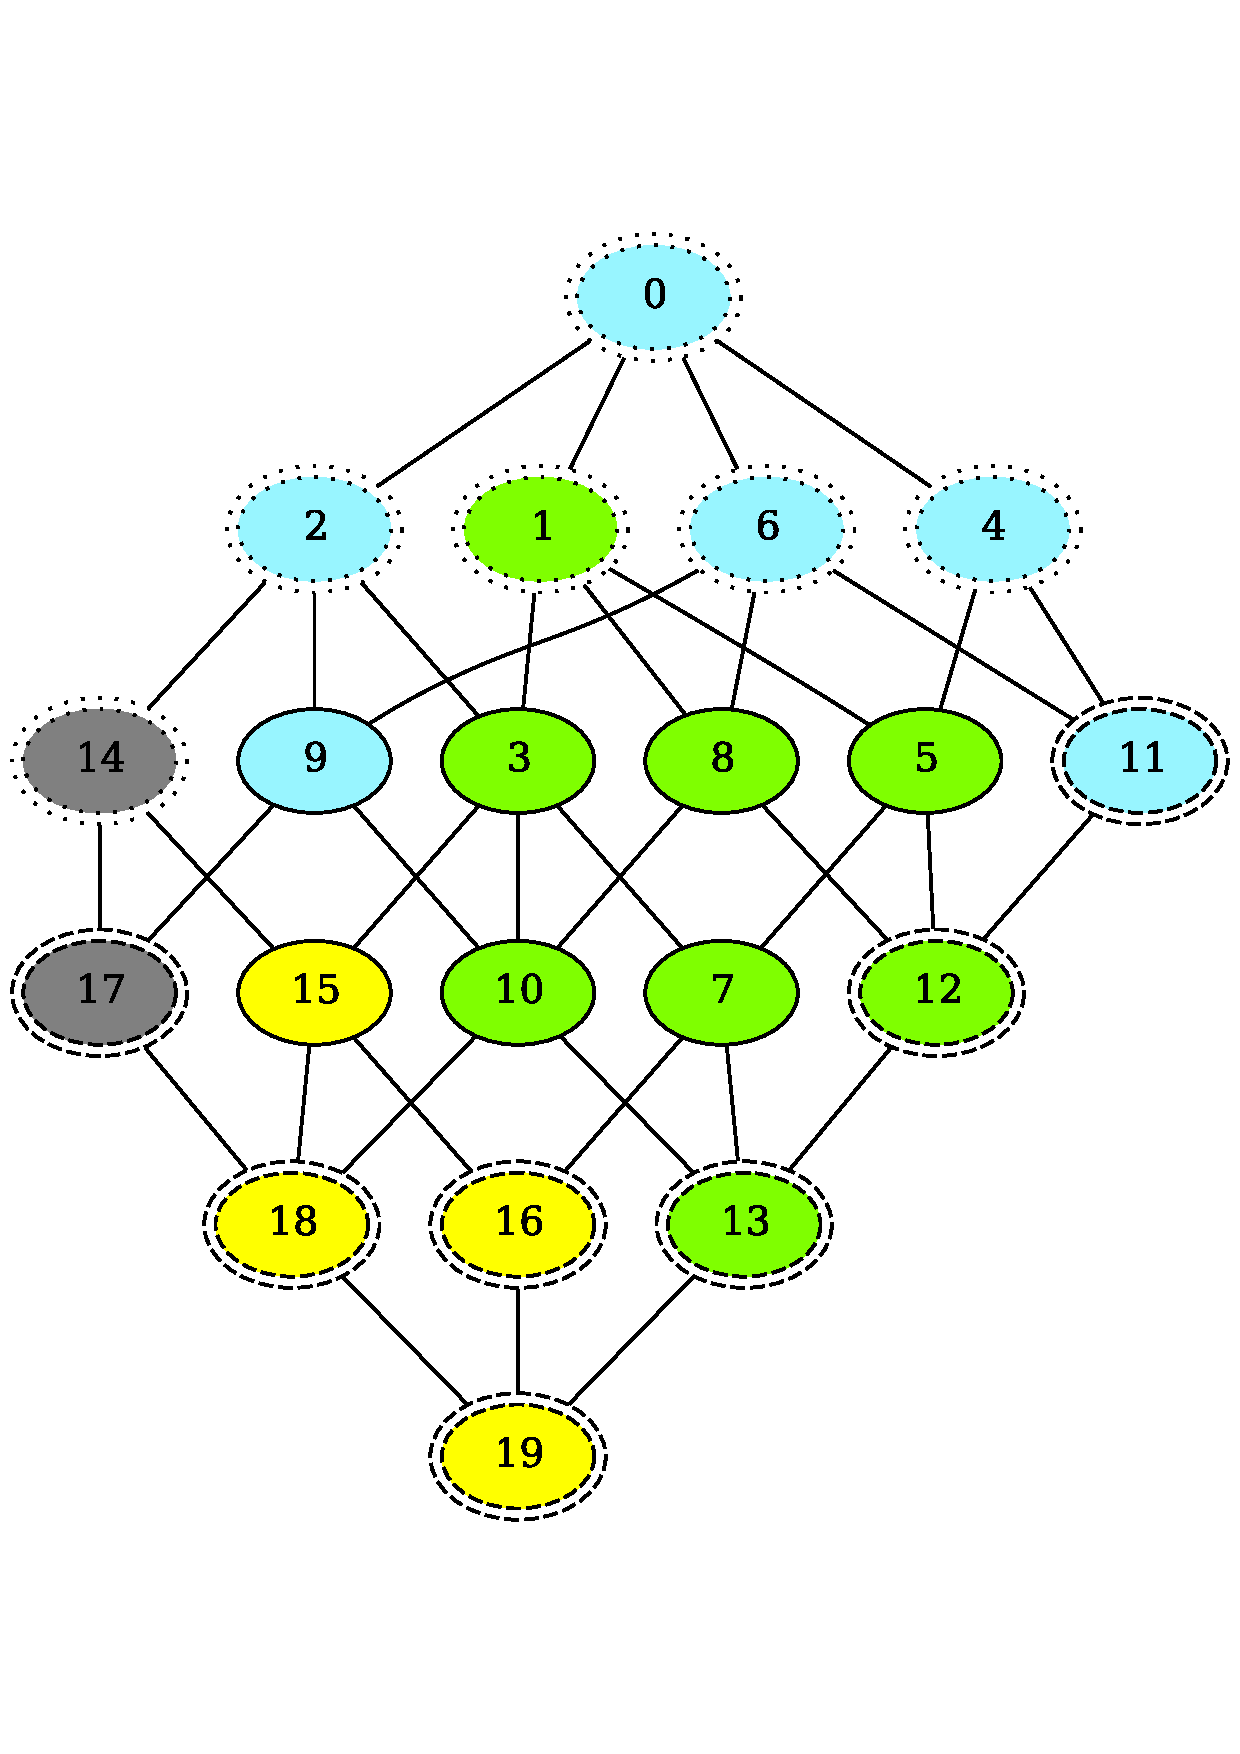
\includegraphics[scale=0.25]{g-12-1.pdf}}&
    \imagetop{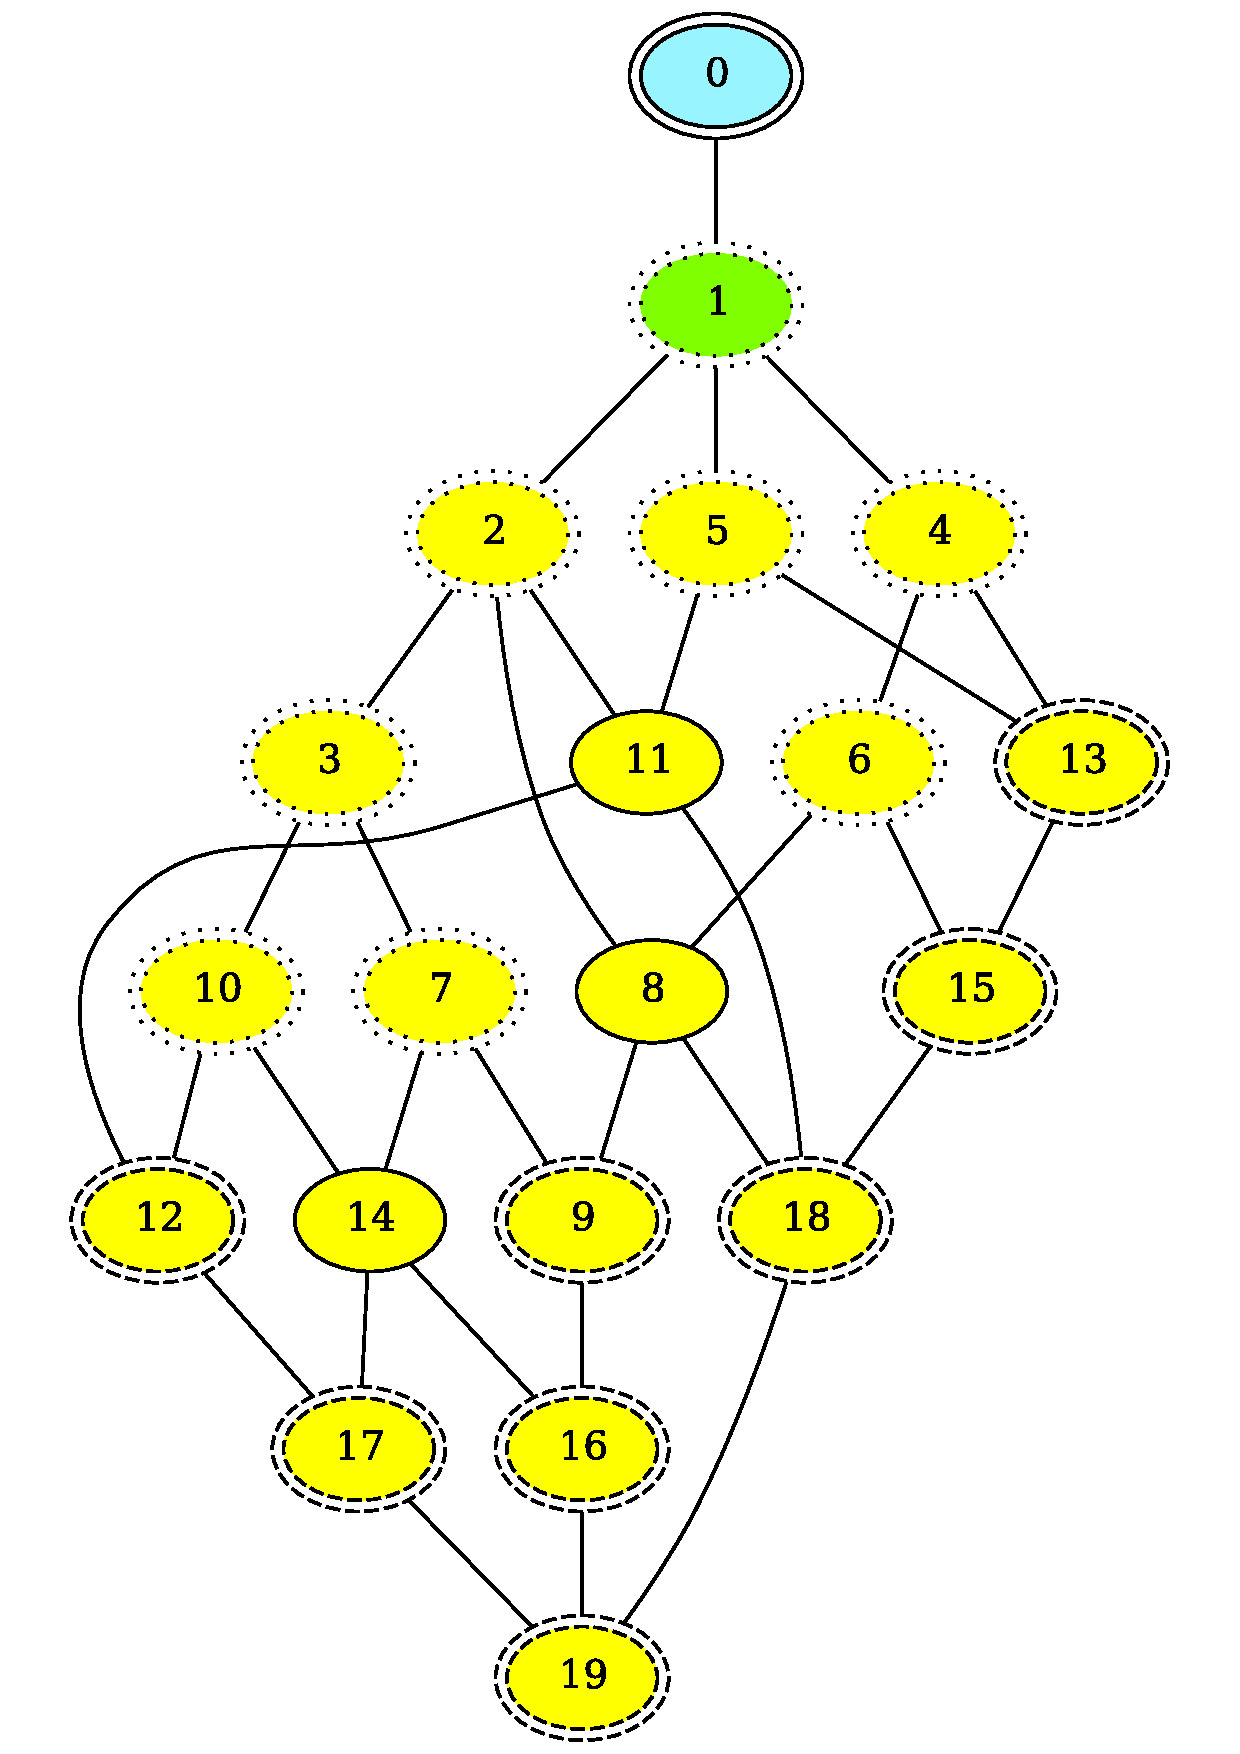
\includegraphics[scale=0.25]{g-A-5.pdf}}&
    \imagetop{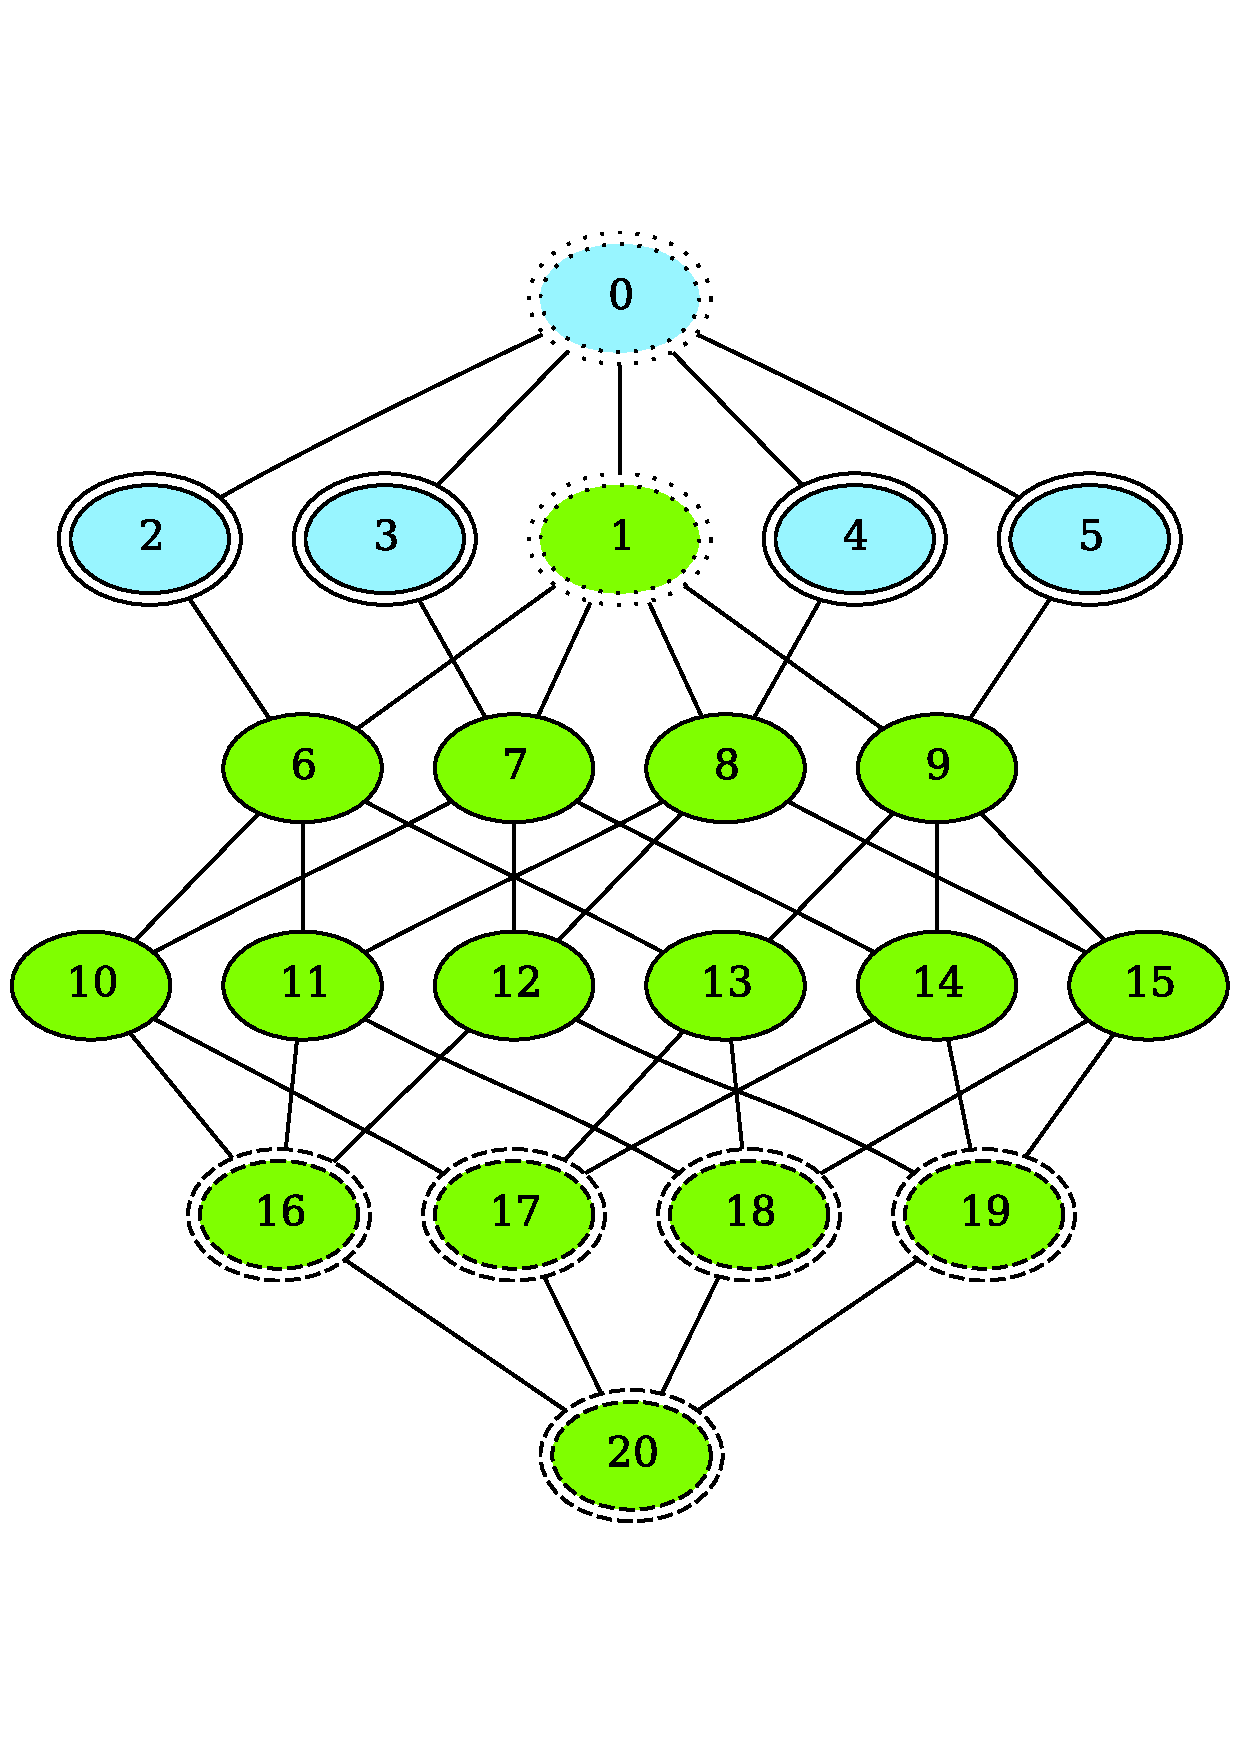
\includegraphics[scale=0.24]{g-9-2.pdf}}
\end{tabular}

\includegraphics[scale=0.04]{legend.png}
\end{center}	
   }
 %%%%%%%%%%%%%%%%%%%%%%%%%%%%%%%%%%%%%%%%%%%%%%%%%%%%%%%%%%%%%%%%%%%%%%%%%%%%%%
   \headerbox{Process}{name=process,column=1}{
 %%%%%%%%%%%%%%%%%%%%%%%%%%%%%%%%%%%%%%%%%%%%%%%%%%%%%%%%%%%%%%%%%%%%%%%%%%%%%%
          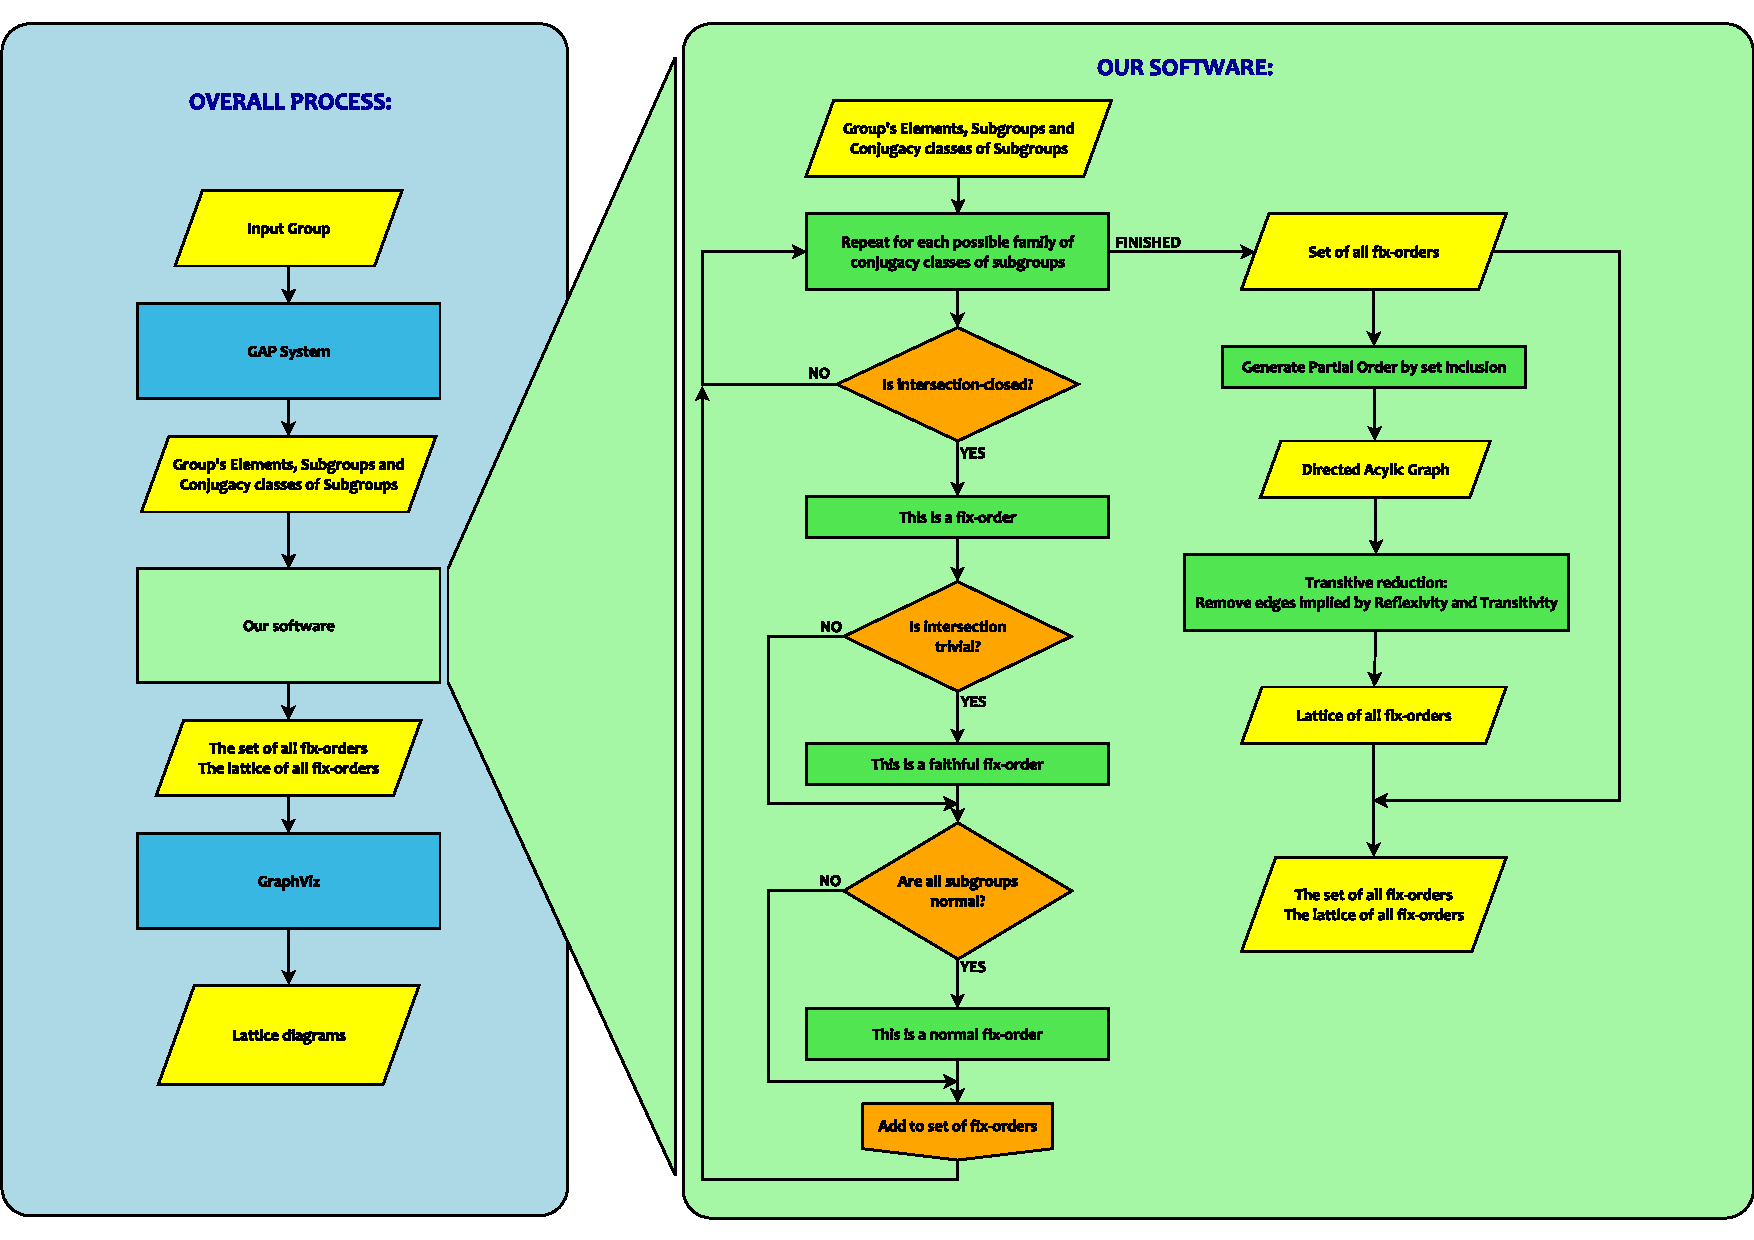
\includegraphics[width=\linewidth]{process2.pdf}
   }
 %%%%%%%%%%%%%%%%%%%%%%%%%%%%%%%%%%%%%%%%%%%%%%%%%%%%%%%%%%%%%%%%%%%%%%%%%%%%%%
   \headerbox{Outcomes}{name=outcomes,column=1, below=process}{
 %%%%%%%%%%%%%%%%%%%%%%%%%%%%%%%%%%%%%%%%%%%%%%%%%%%%%%%%%%%%%%%%%%%%%%%%%%%%%%
The outcomes of this project are:
   \begin{list}{$\bullet$}{}
	\item Complete description of the lattice of fix-orders of all groups of order 15 or less, including:
		\begin{list}{$\circ$}{}
		\item Faithfulness and normality of the fix-orders.
		\item Modularity and Distributivity of the lattice of fix-orders.
		\item The join irreducible and meet irreducible fix-orders of the lattice.
		\item The fix-orders related by an automorphism transformation in the lattice.
		\end{list}
	\item Description of the fix orders of some selected Dihedral, Symmetric and Alternating Groups as well as some groups of order 31 or less. Approximately 120 groups have been processed.
	\item A software package which is able to determine the lattice of fix-orders for any input group, in $O(2^N)$, where N is the number of conjugacy classes of subgroups.
	\end{list}	
   }

 %%%%%%%%%%%%%%%%%%%%%%%%%%%%%%%%%%%%%%%%%%%%%%%%%%%%%%%%%%%%%%%%%%%%%%%%%%%%%%
   \headerbox{Open Problems}{name=openqs,column=1,above=bottom}{
 %%%%%%%%%%%%%%%%%%%%%%%%%%%%%%%%%%%%%%%%%%%%%%%%%%%%%%%%%%%%%%%%%%%%%%%%%%%%%%
     In general, lattice distributivity is a stronger condition than lattice modularity. However, in all of the lattices of fix-orders we examined, distributivity and modularity were equivalent. It is not known whether this holds for all lattices of fix-orders.
   }

 %%%%%%%%%%%%%%%%%%%%%%%%%%%%%%%%%%%%%%%%%%%%%%%%%%%%%%%%%%%%%%%%%%%%%%%%%%%%%%
   \headerbox{References}{name=references,column=0,below=aim}{
 %%%%%%%%%%%%%%%%%%%%%%%%%%%%%%%%%%%%%%%%%%%%%%%%%%%%%%%%%%%%%%%%%%%%%%%%%%%%%%
          \small
     
     \bibliographystyle{ieee}
    
     \renewcommand{\section}[2]{\vskip 0.05em}
       \begin{thebibliography}{1}\itemsep=-0.01em
       \setlength{\baselineskip}{0.4em}
	

       \bibitem{} I.~Hawthorn, T.~Stokes, Groups with fix-set quasi-order, in preparation.
       \bibitem{} T.~Stokes, Axioms for function semigroups with agreement quasi-order, Algebra Univ 66 (2011), 85-98.
       \end{thebibliography}
   }

 %%%%%%%%%%%%%%%%%%%%%%%%%%%%%%%%%%%%%%%%%%%%%%%%%%%%%%%%%%%%%%%%%%%%%%%%%%%%%%
   \headerbox{Acknowledgements}{name=ack,column=0,above=bottom}{
 %%%%%%%%%%%%%%%%%%%%%%%%%%%%%%%%%%%%%%%%%%%%%%%%%%%%%%%%%%%%%%%%%%%%%%%%%%%%%%
    Thanks to the University of Waikato Summer research programme for the opportunity to work on this project.
   }

\end{poster}%
%
\end{document}
